\section{Introduction}
\label{sec:introduction}

Modern neural networks are both expressive and accurate over a wide variety of learning and classification problems, but at the cost of increased width and depth. State-of-the-art convolutional models, for example, can contain up to several billion parameters \citep{khan2020survey,szegedy2015going, brown2020language}. The size and training costs of such networks are at odds with a rapidly emerging industrial and academic interest in performing learning tasks on low-fidelity hosts such as IoT and mobile devices \citep{mcmahan2017communication,li2018learning,kairouz2019advances}.

An increasingly popular approach for generating compact yet expressive models is to use Tensorial Neural Networks (TNNs) \citep{lebedev2015speeding, kossaifi2017tensor, kossaifi2020tensor,su2018tensorial}, which factorize each layer’s weight tensor into several smaller factors.
As a result, each TNN layer is a multilinear operation among its input and weight factors.

One particular method by which a TNN can arise is reshaping a network weight into a higher order tensor. These reshaped weights are then decomposed into factorized forms, such as canonical polyadic (CP), tensor train (TT), and Tucker (TK) decompositions. Factorization of a reshaped tensor is an efficient way of representing underlying properties such as periodicity and modularity invariances/similarities, which often exist in neural network models \citep{lebedev2015speeding, garipov2016ultimate, su2018tensorial,wang2018wide}, and preserved in the factorization. This is especially useful for low-rank, higher-order reshaped weights since we can capture abundant structural information without much representation redundancy. \Cref{fig:periodicity} depicts this scenario using the example of a vector displaying periodicity.

% Figure for reshaping
\begin{figure}[!htbp]
    \vspace{-0.5em}
    \centering
    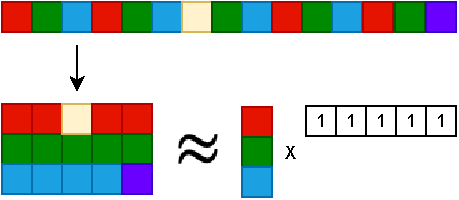
\includegraphics[width=0.3\textwidth]{\fighome/modularity.pdf}
    \vspace{-0.5em}
    \caption{\textbf{Tensor reshaping.} 
    The figure shows how reshaping can help reduce the number of parameters while preserving critical structural properties. A vector of length 15 displays periodicity in its entries (represented here by repeating colors) except for a few entries. Reshaping it into a $3\times 5$ matrix and then taking a factorized tensor approximation (rank-1 SVD) \textbf{a)} reduces the number of parameters to store and \textbf{b)} culls out artifacts (non-periodic elements) while representing periodicity sans redundancy.
    }
\label{fig:periodicity}
\vspace{-1em}
\end{figure}

In addition to the lighter weight, TNNs preserve the same predictive power level over various backbone networks and tasks. However, in contrast to the availability of high-performance libraries for convolutional neural networks (CNNs) (e.g., NVIDIA’s cuDNN for GPUs, Intel’s MKL for CPUs), efficient library-based solutions are not available for training TNNs, especially those based on CNNs.

In this work, we introduce an open-source library and a suite of meta-algorithms, collectively termed as \autotnn, to efficiently construct and train TNNs. Given a backbone network, \autotnn will tensorize its layers, compress the tensorial weights, and conduct end-to-end training on the resulting TNN. In particular, the user does not need to develop any part of the TNN architecture on their own. 

\autotnn interprets the forward and backward pass of a TNN as a \textit{generalized} \einsum graph/sequence. Here, ``generalized'' means including convolutions, an operation not supported by any existing \einsum implementation but handled by our meta-function \conveinsum. A lack of support for convolution operations in $\einsum$ prevented the evaluation of tensorized CNNs via well-known algorithms such as \netcon. However, deriving tensor decompositions with convolutions is nontrivial as (a) the factorization involving a convolution is challenging to represent as an einsum string, and (b) backpropagation rules for such structure designs were not derived in any prior work. \conveinsum evaluates these tensor operations with an optimal sequence, rather than naively performing all the tensor operations from left to right, resulting in a vastly reduced/improved number of \emph{floating point operations} (FLOPs) during training and inference, a mechanism we refer to as the \textit{optimal sequencer}.

In totality, \autotnn addresses computational and memory overhead challenges associated with automated TNN construction and training. In conjunction with $\conveinsum$, the optimal sequencer, and checkpointing, this work provides a framework and library which significantly improves the efficiency of TNN design and deployment.

\textbf{Summary of contributions.} \\
\textbf{(1)} We develop an open-source library \autotnn and framework for designing and training a TNN given a backbone network and specified tensor decomposition. \\
\textbf{(2)} Our algorithm \conveinsum optimizes the training process. In particular, \conveinsum interprets forward and backward passes as sequences of multi-linear operations, including multi-way (and thus multi-linear) convolutions, thereby extending the classical \einsum. \\
\textbf{(3)} Furthermore, \conveinsum utilizes the library \opteinsum \citep{daniel2018opt}, which generalizes the \netcon algorithm \citep{pfeifer2014faster}, to efficiently determine an optimal evaluation order of these sequences. \\
\textbf{(4)}  We exploit a mechanism referred to as \textit{checkpointing} \citep{chen2016training} which can balance the computational cost of a forward or backward pass of a TNN with the memory cost of large intermediate products during evaluation.\\
\textbf{(5)}  Our experiments demonstrate the expressiveness of TNNs with \autotnn over various tasks including video classification, speech-recognition, and image classification. 

%\textbf{(1)}  We develop an open-source library and framework \autotnn which is capable of building and training a TNN given a backbone network and specified tensor decomposition.
%\textbf{(2)} Our API \conveinsum optimizes the training process. In particular, \conveinsum interprets forward and backward passes as sequences of multi-linear operations, including multi-way (and thus multi-linear) convolutions, thereby extending the classical \einsum.
%\textbf{(3)} Furthermore, \conveinsum utilizes the library \opteinsum \citep{daniel2018opt}, which generalizes the \netcon algorithm \citep{pfeifer2014faster}, to efficiently determine an optimal evaluation order of these sequences. 
%\textbf{(4)} We exploit a mechanism referred to as \textit{checkpointing} \citep{chen2016training} which can balance the computational cost of a forward or backward pass of a TNN with the memory cost of large intermediate products during evaluation.
%\textbf{(5)} Our experiments demonstrate the expressive power of TNNs constructed via \autotnn over a large domain of tasks including video classification, speech-recognition, and image classification. 


%\tr{We stress, however, that the purpose of our experimental work is not to demonstrate the SOTA accuracy of TNNs over various tasks; this has been shown in prior literature \citep{lebedev2015speeding, kim2015compression, wang2017tensor, su2018tensorial, hayashi2019exploring, lee2021qttnet} via hard-coded TNN architectures in combination with other compression methods (such as pruning, knowledge distillation, quantization, etc.). 